\chapter{Validación y pruebas}
\label{cap:validacion_pruebas}

Una vez implementadas las estaciones de campo y el sistema de supervisión en Raspberry Pi, se ha realizado una validación progresiva del prototipo TierraViva.

Además de las pruebas de laboratorio y de integración controlada, se incluye una prueba funcional en entorno real en Agrolab Móstoles, situado en Móstoles, Madrid. Agrolab se utiliza como entorno de validación por tratarse de un espacio de agricultura urbana/periurbana, más próximo al contexto de uso previsto que el montaje inicial de laboratorio \cite{ayto_mostoles_agrolab_2020}. Esta prueba permite comprobar el comportamiento del prototipo en una zona de cultivo real y obtener evidencia audiovisual del funcionamiento de la estación, la publicación de datos y la actuación controlada del riego.

El plan completo de pruebas, criterios de aceptación y relación con riesgos técnicos, se recoge en el Anexo~\ref{anexo:plan_pruebas}. La relación entre requisitos, pruebas y evidencias se documenta de forma complementaria en el Anexo~\ref{anexo:trazabilidad_requisitos_pruebas}. En este capítulo se presenta únicamente la síntesis de validación necesaria para evaluar el funcionamiento global del prototipo.

\section{Estrategia de validación}
\label{sec:estrategia_validacion}

La validación se ha organizado de forma incremental, desde componentes aislados hasta el flujo completo extremo a extremo. Esta estrategia evita que los errores de alimentación, cableado, comunicación o software aparezcan únicamente al final, cuando resulta más difícil aislar su origen. La Figura~\ref{fig:estrategia_incremental_validacion} resume los niveles aplicados.

\begin{figure}[H]
    \centering
    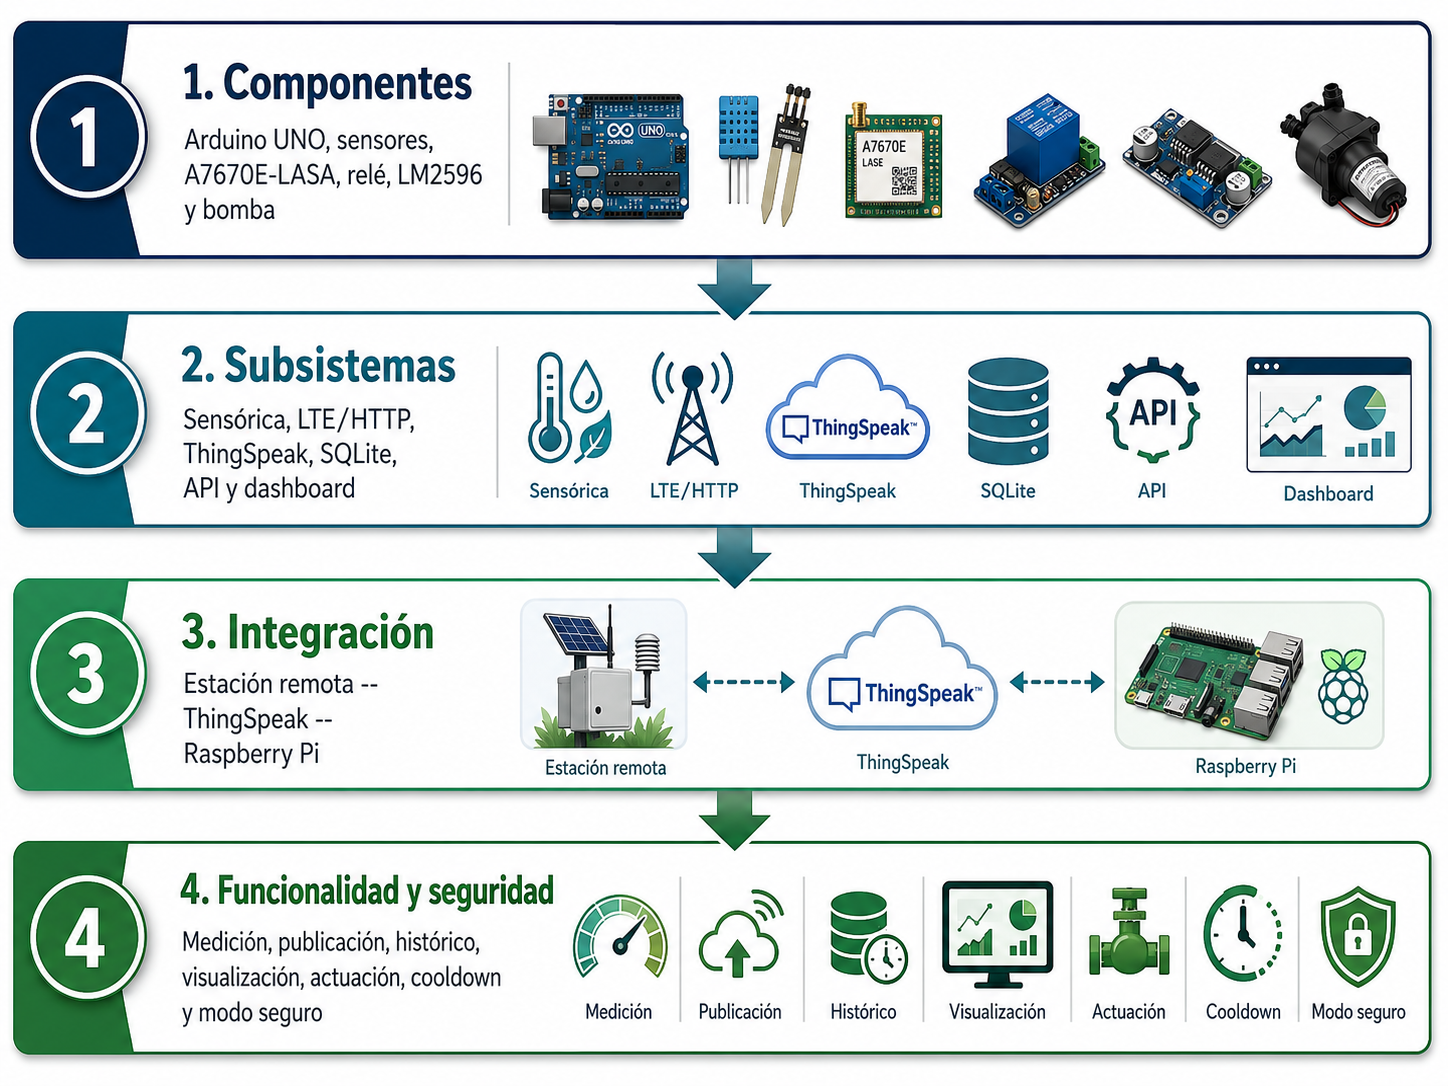
\includegraphics[width=\textwidth]{figs_png/estrategia_incremental_validacion.png}
    \caption{Estrategia incremental de validación aplicada en TierraViva. Elaboración propia, véase Anexo~\ref{sec:uso_ia_generativa_tfg}.}
    \label{fig:estrategia_incremental_validacion}
\end{figure}

La validación se interpreta como una comprobación técnica del prototipo desarrollado. El objetivo es demostrar que la arquitectura propuesta funciona, que los bloques se comunican correctamente y que la actuación sobre el riego incorpora medidas básicas de seguridad.

\section{Resumen de pruebas realizadas}
\label{sec:resumen_pruebas_realizadas}

La Tabla~\ref{tab:cap7_resumen_pruebas} resume las pruebas principales ejecutadas durante la validación. Se han agrupado siguiendo la numeración definida en el Anexo~\ref{anexo:plan_pruebas}, pero evitando repetir el detalle procedimental de cada caso.

\begin{table}[H]
\centering
\scriptsize
\renewcommand{\arraystretch}{1.15}
\rowcolors{2}{TableRowSoft}{white}
\begin{tabular}{|p{0.10\textwidth}|p{0.25\textwidth}|p{0.35\textwidth}|p{0.18\textwidth}|}
\hline
\rowcolor{URJCRed}
\TVHead{Prueba} & \TVHead{Bloque validado} & \TVHead{Resultado obtenido} & \TVHead{Estado} \\
\hline
P01 & Alimentación y masa común & Se verificó la alimentación principal de 12 V, la regulación a 5 V mediante LM2596 y la referencia común de masa entre bloques. & Superada \\
\hline
P02--P04 & Sensores & Se validó BME280, BH1750 y sensor capacitivo de humedad de suelo mediante lectura individual y conjunta. & Superadas \\
\hline
P05 & A7670E-LASA por USB & El módem respondió a comandos AT, reconoció la SIM, obtuvo señal, registró red y permitió comunicación HTTP. & Superada \\
\hline
P06 & Publicación en ThingSpeak & La estación publicó telemetría y estado en el canal ThingSpeak correspondiente mediante LTE/HTTP. & Superada \\
\hline
P07--P08 & Raspberry Pi y SQLite & La Raspberry consultó datos de ThingSpeak, evitó duplicados mediante \texttt{entry\_id} y registró lecturas en SQLite. & Superadas \\
\hline
P09 & API FastAPI & Los \textit{endpoints} de consulta devolvieron datos coherentes con la base de datos local. & Superada \\
\hline
P10 & \textit{dashboard} web & La interfaz mostró lecturas, estado de conexión, gráficas, histórico y selección de estación. & Superada \\
\hline
P11 & Relé sin bomba & Se comprobó la conmutación del relé y el retorno a estado apagado sin carga hidráulica. & Superada \\
\hline
P12 & Bomba de agua & Se validó la activación temporizada de la bomba y su apagado explícito al finalizar el intervalo de riego. & Superada \\
\hline
P13--P15 & Seguridad funcional & Se comprobaron \textit{cooldown}, rechazo de lecturas no válidas y comportamiento seguro ante pérdida temporal de comunicación. & Superadas \\
\hline
P16 & Integración completa & Se validó el flujo extremo a extremo: estación, ThingSpeak, Raspberry Pi, SQLite, API, \textit{dashboard} y actuación local. & Superada \\
\hline
P17 & Prueba funcional en Agrolab Móstoles & Se validó el funcionamiento del prototipo en un entorno real de cultivo, documentando el montaje, la publicación de telemetría, la visualización y la actuación controlada mediante evidencia fotográfica y vídeo. & Superada \\
\hline
\end{tabular}
\caption{Resumen de pruebas principales realizadas en TierraViva.}
\label{tab:cap7_resumen_pruebas}
\end{table}

El resultado global de las pruebas es positivo: los bloques esenciales del sistema han sido implementados y validados de forma integrada. Las observaciones más relevantes corresponden a limitaciones propias de esta primera versión: necesidad de una calibración agronómica más precisa del sensor de humedad de suelo, dependencia de cobertura LTE, consumo del módulo celular y conveniencia de una validación prolongada en entorno real durante más tiempo.

\section{Validación de la estación remota}
\label{sec:validacion_estacion_remota}

La estación remota se validó primero como montaje físico completo. La Figura~\ref{fig:foto_estacion_validacion} muestra el prototipo empleado durante las pruebas, integrando Arduino UNO, sensores, módulo A7670E-LASA, relé, alimentación regulada y bomba de agua.

\begin{figure}[H]
    \centering
    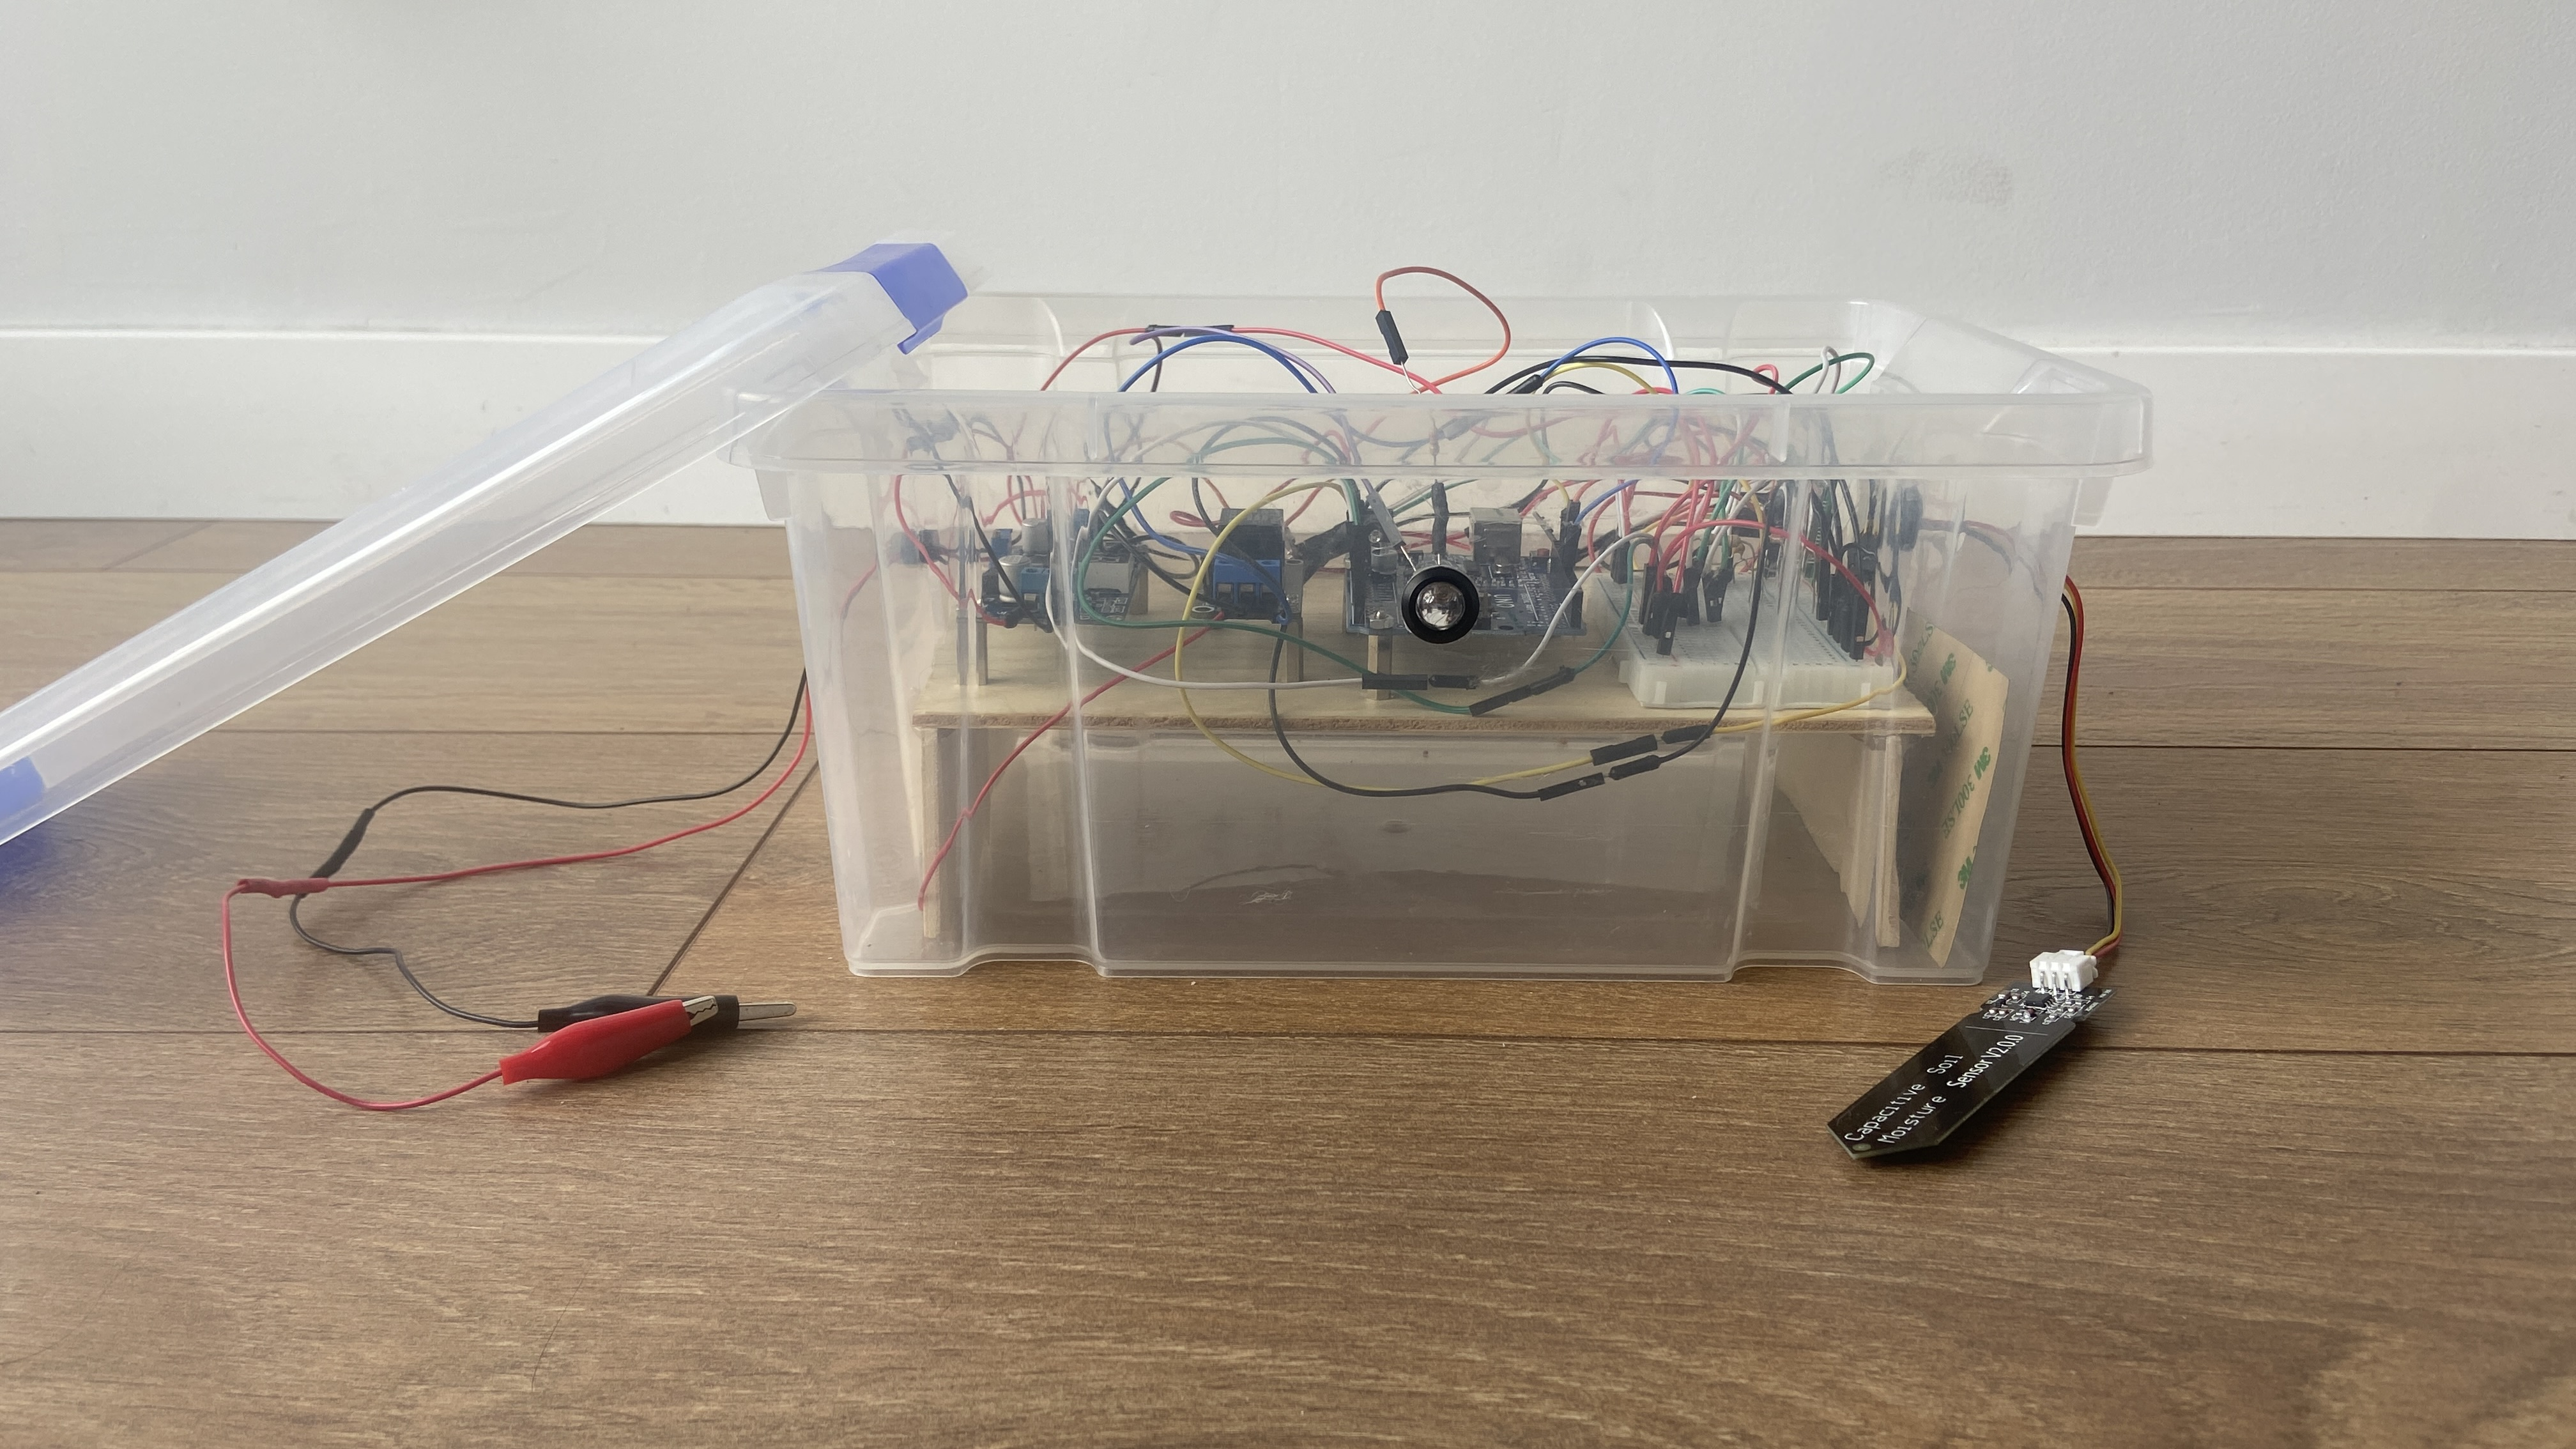
\includegraphics[width=0.82\textwidth]{figs/foto_estacion_validacion.jpg}
    \caption{Montaje físico utilizado para la validación de la estación remota (!!!!!cambiar por la definitiva!!!!!). Elaboración propia.}
    \label{fig:foto_estacion_validacion}
\end{figure}

La primera comprobación fue la programación del Arduino UNO compatible. Tras instalar el controlador del conversor \texttt{CH340G}, la placa fue reconocida en Windows como puerto \texttt{COM3} y se validó la carga del ejemplo \textit{Blink}. Con ello quedó comprobada la cadena básica de programación: detección USB, selección de placa, compilación, carga y ejecución.

Después se validó el bloque de sensórica. El escaneo I2C detectó el BH1750 en \texttt{0x23} y el BME280 en \texttt{0x76}, confirmando que ambos sensores podían compartir las líneas \texttt{A4/SDA} y \texttt{A5/SCL}. El sensor capacitivo de humedad de suelo se comprobó mediante lectura analógica en \texttt{A0}, observándose variaciones claras al modificar las condiciones de contacto del sensor.

Finalmente, se ejecutó el \textit{firmware} conjunto de estación. Esta prueba confirmó que el Arduino podía leer humedad de suelo, temperatura, humedad relativa, presión y luminosidad en un mismo ciclo, actualizar su estado interno y dejar preparada una muestra completa de telemetría para su publicación.

La actuación se validó de forma progresiva: primero mediante relé e indicador visual, y después con la bomba de agua de 12 V como carga real. La prueba confirmó que el \textit{firmware} activa el relé durante un intervalo limitado y lo apaga explícitamente al finalizar.

\section{Validación de comunicación, ThingSpeak y supervisión}
\label{sec:validacion_comunicacion_supervision}

La comunicación remota se validó primero de forma independiente y después integrada con Arduino. El A7670E-LASA respondió correctamente a comandos AT desde ordenador, reconoció la SIM, obtuvo señal, registró red LTE y permitió ejecutar peticiones HTTP. Posteriormente, el módem se conectó al Arduino mediante \texttt{SoftwareSerial}, trabajando a \texttt{9600} baudios para priorizar estabilidad.

La publicación en ThingSpeak se consideró válida cuando la estación obtuvo una respuesta HTTP correcta y los datos aparecieron en el canal correspondiente. Cada envío incluye humedad de suelo, temperatura, humedad relativa, luminosidad, presión, estado del relé, evento de sistema y código auxiliar de diagnóstico. La estructura completa de campos y códigos se documenta en el Anexo~\ref{anexo:estructura_thingspeak_estados}.

La Raspberry Pi se validó consultando los canales ThingSpeak, evitando duplicados mediante \texttt{entry\_id}, registrando lecturas en SQLite y exponiendo los datos mediante FastAPI. El \textit{dashboard} confirmó la visualización final de las lecturas, el estado de conexión, la antigüedad del dato, gráficas históricas y selección de estación.

La Figura~\ref{fig:evidencias_validacion_tierraviva} recoge cuatro evidencias visuales del flujo completo de validación: publicación en ThingSpeak, visualización en el \textit{dashboard}, inicialización de la estación desde monitor serie y ciclos de decisión local de riego. Esta composición permite conservar evidencia experimental real sin duplicar figuras extensas en el cuerpo principal de la memoria.

\begin{figure}[H]
\centering

\begin{minipage}{0.48\textwidth}
    \centering
    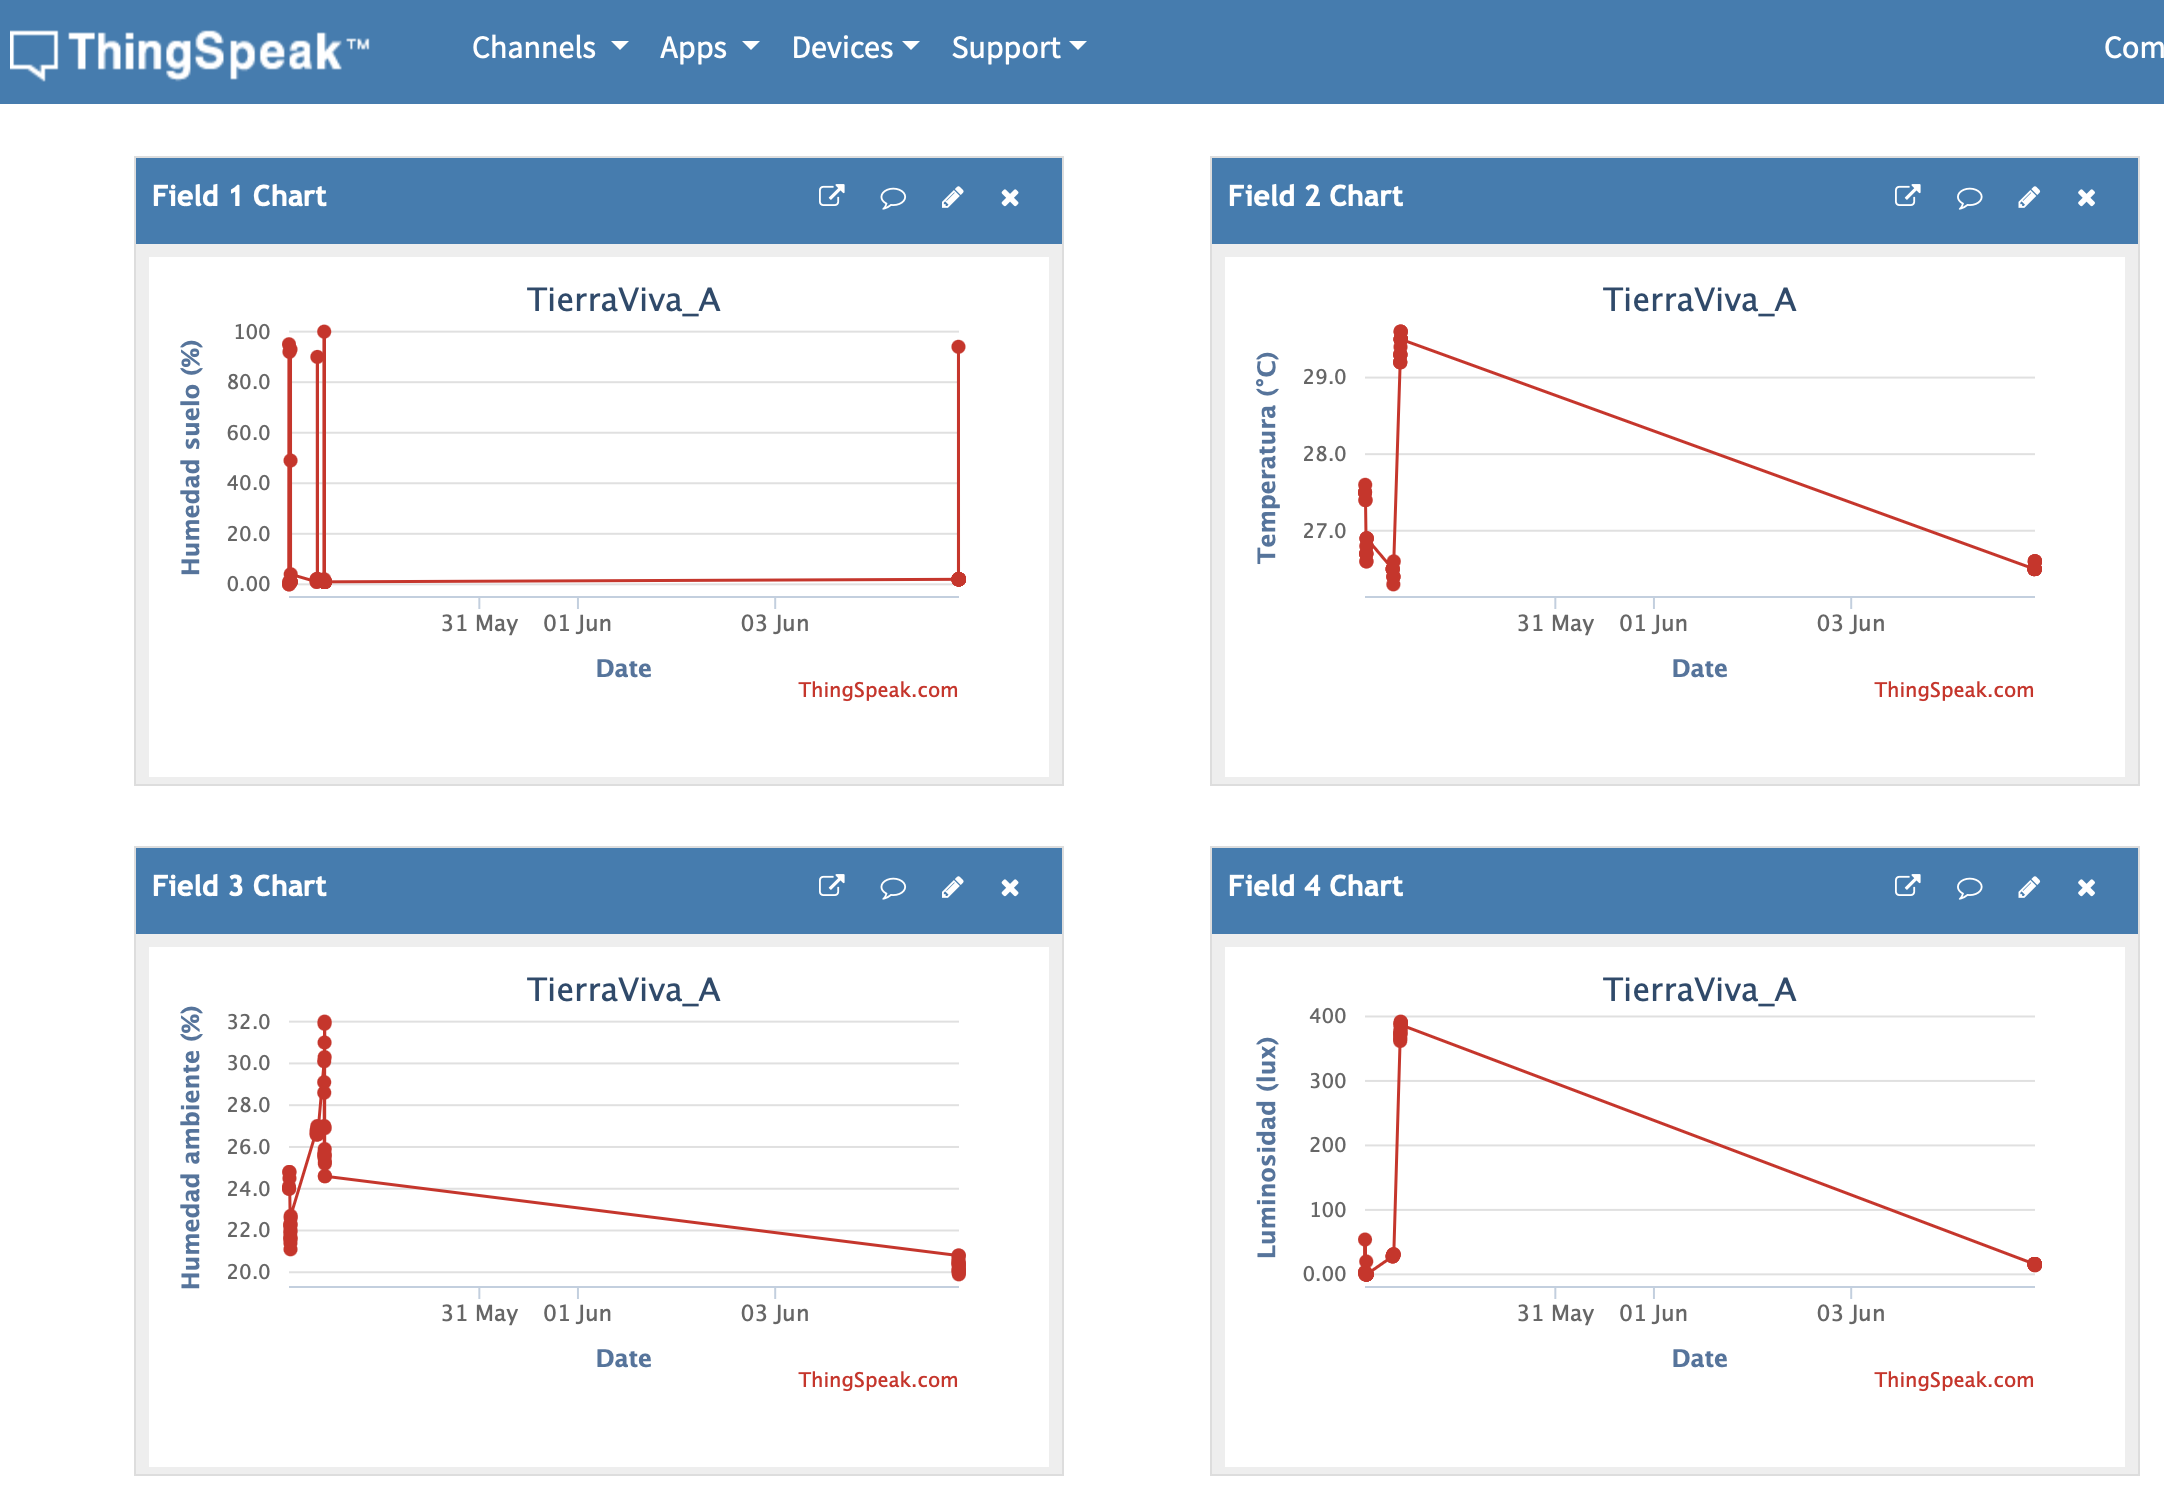
\includegraphics[width=\textwidth]{figs_png/evidencia_thingspeak_publicacion.png}
    \small (a) Publicación de telemetría en ThingSpeak.
\end{minipage}
\hfill
\begin{minipage}{0.48\textwidth}
    \centering
    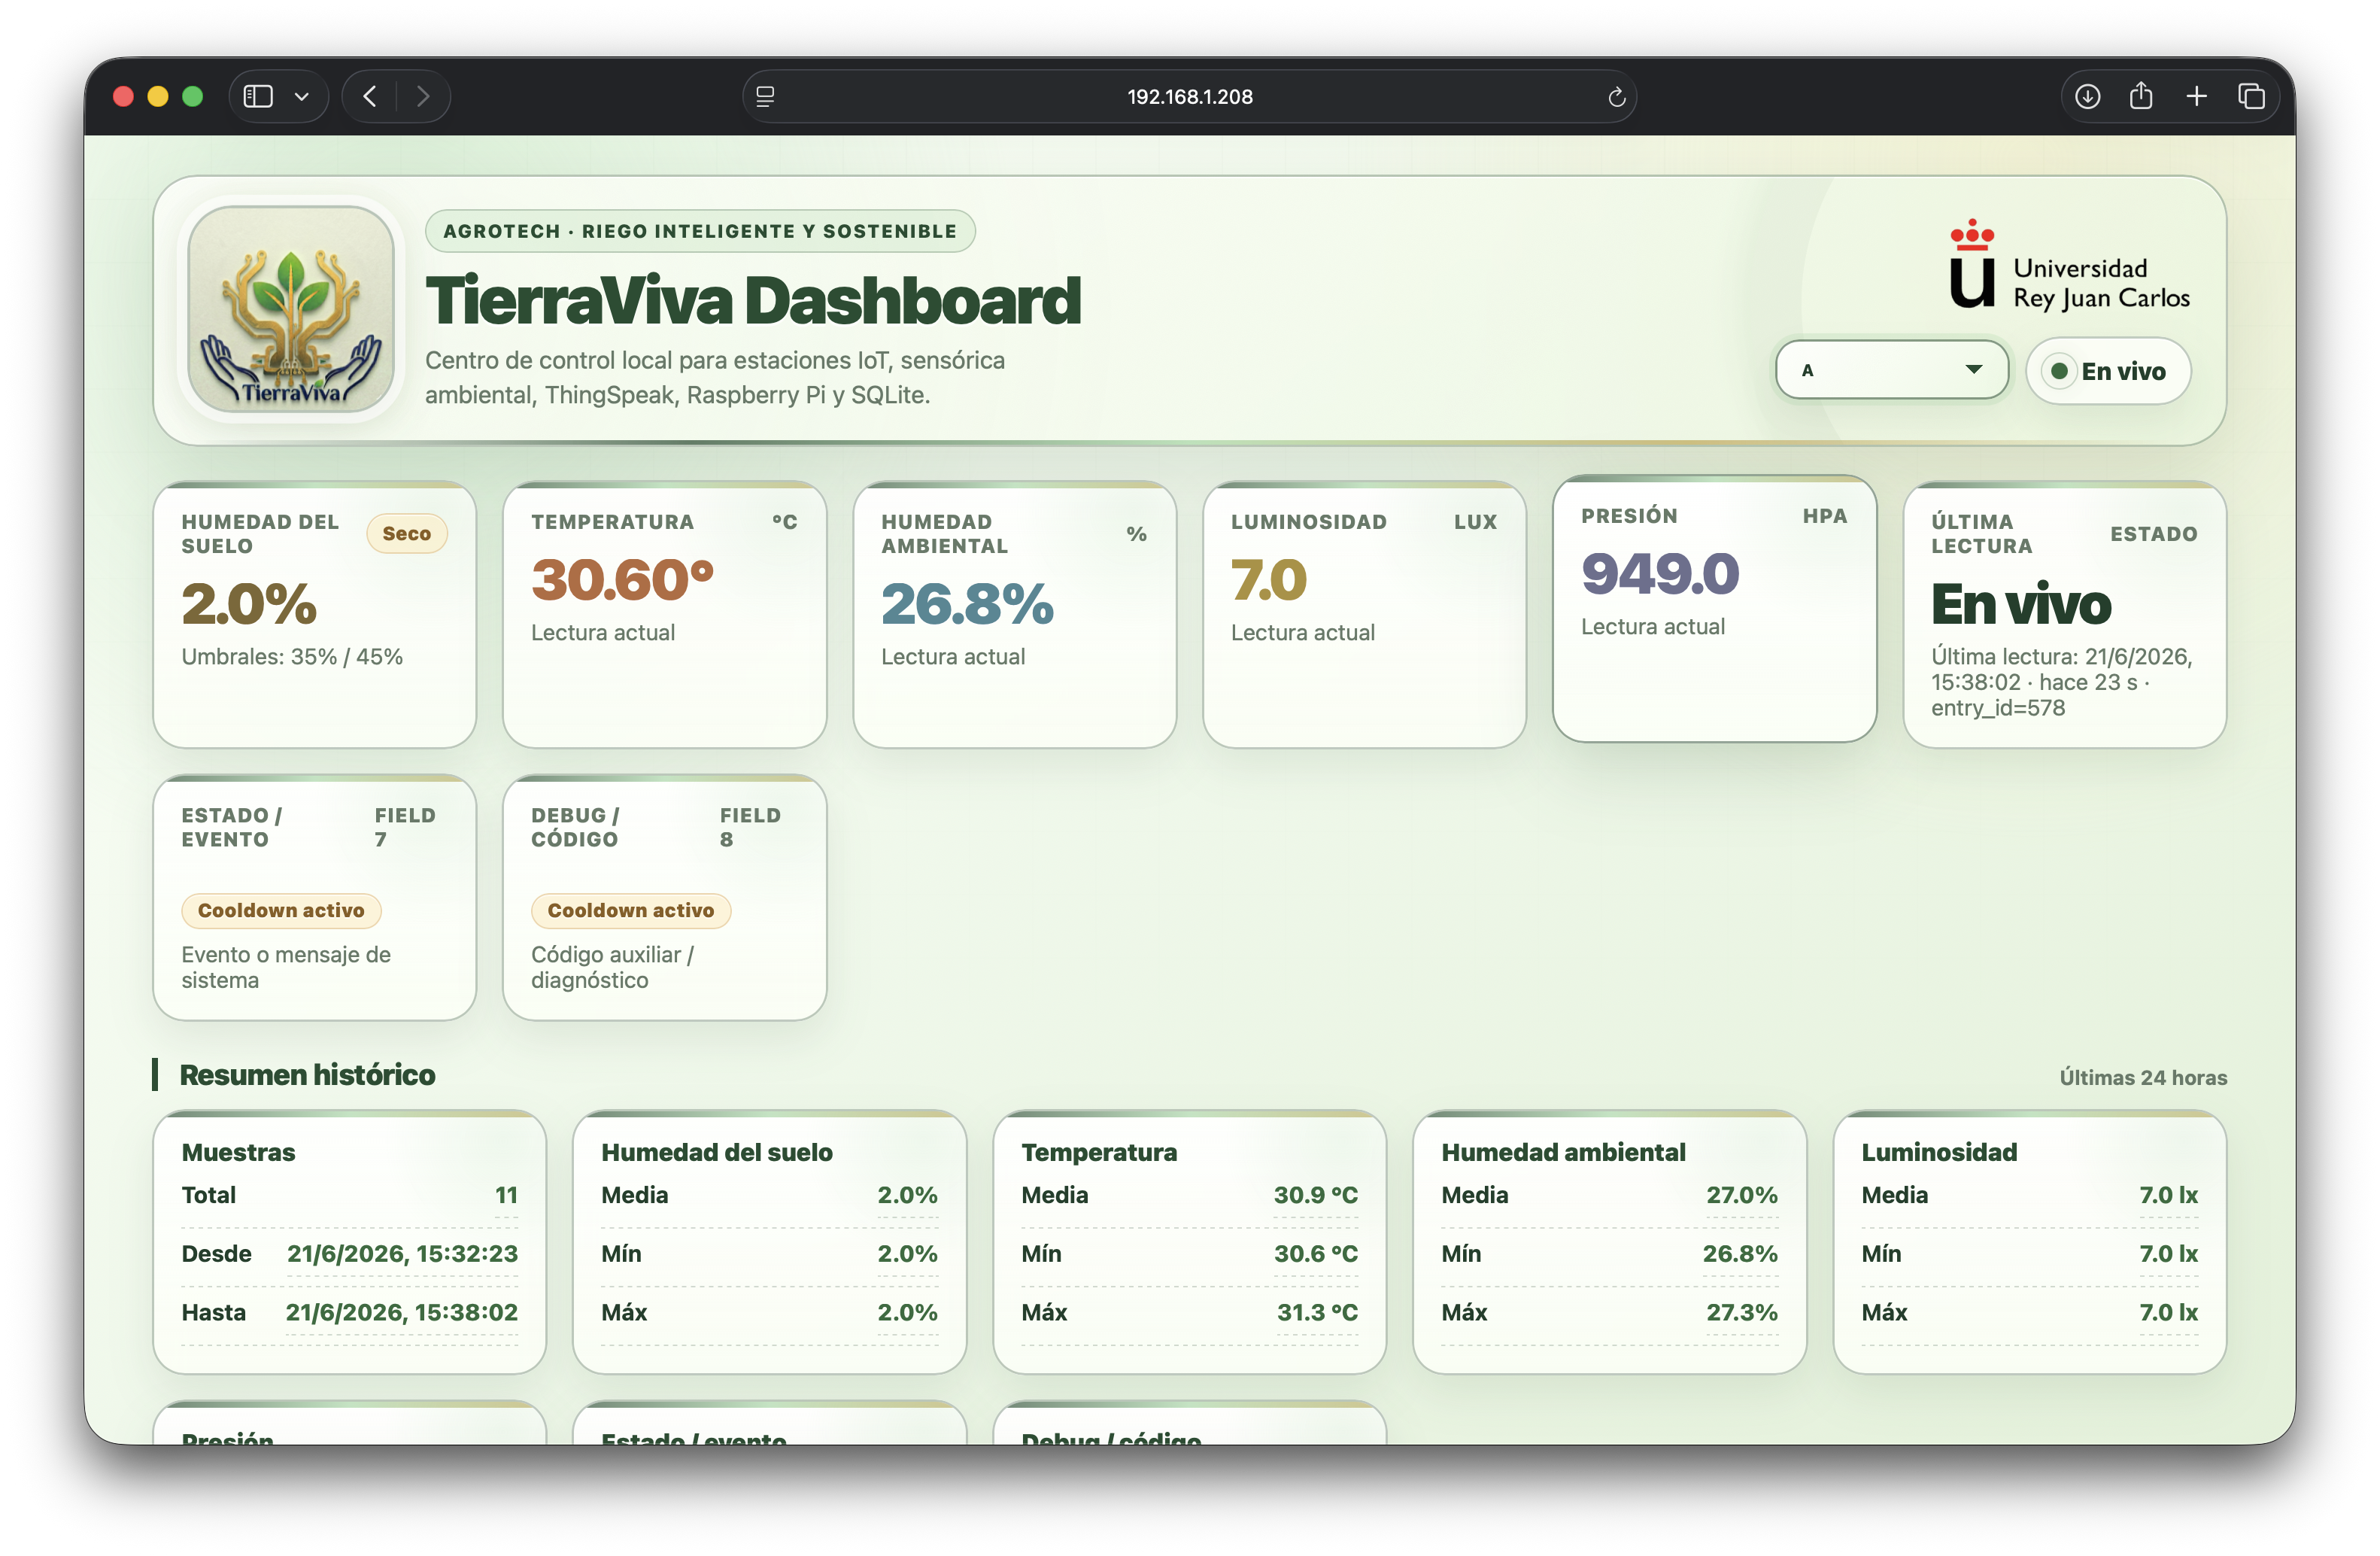
\includegraphics[width=\textwidth]{figs_png/evidencia_dashboard.png}
    \small (b) Visualización en el \textit{dashboard} local.
\end{minipage}

\vspace{0.35cm}

\begin{minipage}{0.48\textwidth}
    \centering
    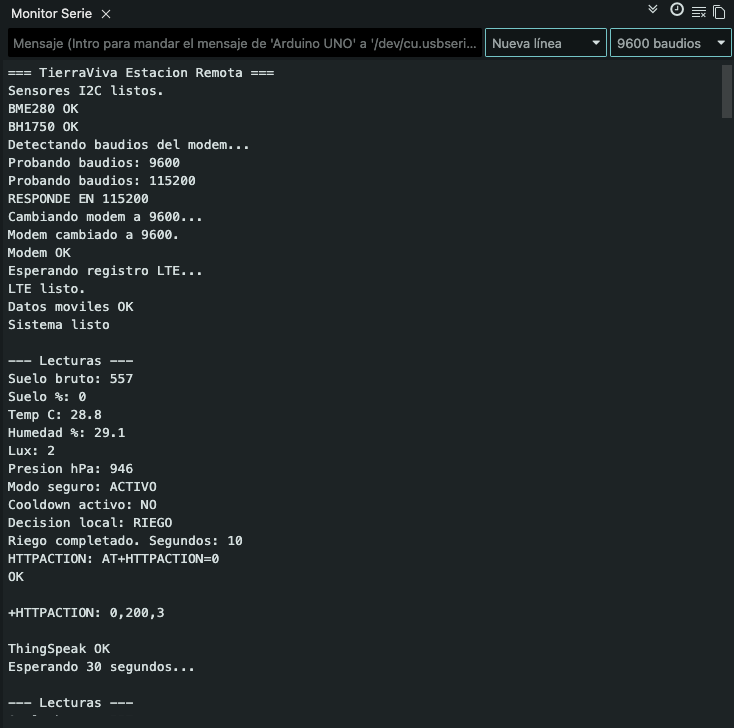
\includegraphics[width=\textwidth]{figs_png/monitor_serie_inicio_lte_thingspeak.png}
    \small (c) Inicialización, registro LTE y publicación HTTP correcta.
\end{minipage}
\hfill
\begin{minipage}{0.48\textwidth}
    \centering
    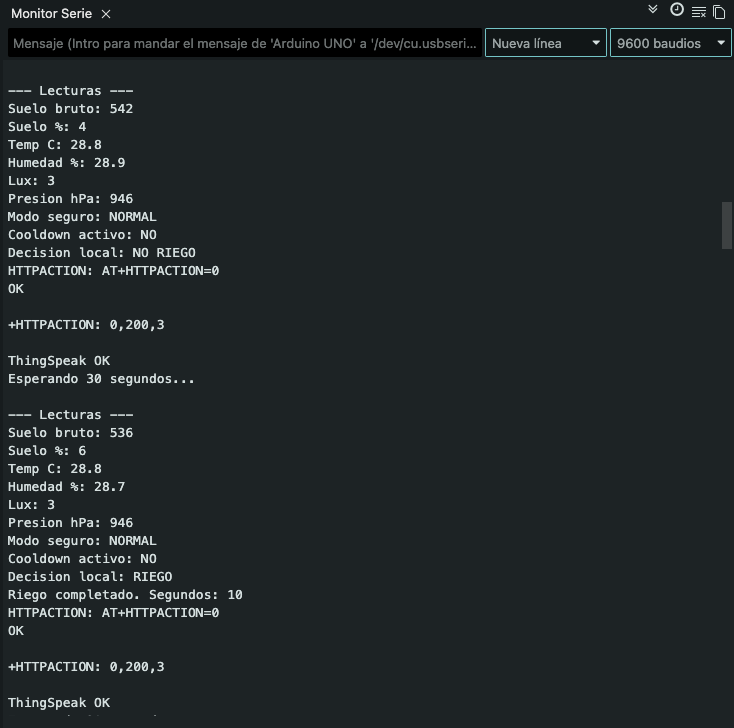
\includegraphics[width=\textwidth]{figs_png/monitor_serie_decision_riego_cooldown.png}
    \small (d) Ciclos de decisión local, riego y \textit{cooldown}.
\end{minipage}

\caption[Evidencias visuales del flujo completo de validación]{Evidencias visuales del flujo completo de validación de TierraViva. Se documenta la publicación de telemetría en ThingSpeak, la visualización desde el \textit{dashboard}, la inicialización de la estación mediante monitor serie y la ejecución de ciclos de decisión local con riego temporizado y bloqueo por \textit{cooldown}. Capturas propias.}
\label{fig:evidencias_validacion_tierraviva}
\end{figure}

Los registros completos asociados a estas capturas se recogen en el Anexo~\ref{subsec:evidencias_monitor_serie_pruebas}.

\section{Prueba funcional en entorno real en Agrolab Móstoles}
\label{sec:validacion_agrolab_mostoles}

Como cierre de la validación, se realizó una prueba funcional en Agrolab Móstoles, un entorno de agricultura urbana/periurbana situado en Móstoles, Madrid. Esta prueba se plantea como una comprobación funcional del prototipo fuera del entorno de laboratorio, orientada a verificar el comportamiento del sistema en una zona de cultivo real.

Durante la prueba se verificó el funcionamiento integrado de la estación de campo, la lectura de sensores, la comunicación LTE, la publicación de telemetría en ThingSpeak, la supervisión desde Raspberry Pi, la visualización en el \textit{dashboard} y la actuación controlada del riego. La prueba permitió comprobar que el sistema mantiene el mismo flujo funcional en un entorno real de cultivo: medir, decidir localmente, actuar de forma temporizada, publicar estado y permitir la supervisión posterior.

\begin{figure}[H]
    \centering
    %
\includegraphics[width=0.82\textwidth]{figs_png/prueba_agrolab_mostoles.png}
    \caption[Prueba funcional de TierraViva en Agrolab Móstoles]{Prueba funcional de TierraViva en Agrolab Móstoles. Vídeo de la prueba disponible en: \url{https://github.com/ltejedorcruz/TierraViva/ENLACE-PENDIENTE-VIDEO-AGROLAB}}
    \label{fig:prueba_agrolab_mostoles}
\end{figure}

La evidencia principal de esta prueba queda formada por la fotografía del montaje en Agrolab, las capturas de ThingSpeak y \textit{dashboard}, y el vídeo de funcionamiento. Por su alcance temporal, la prueba se documenta como validación funcional en entorno real, reservando las campañas agronómicas completas y los ensayos estacionales prolongados para futuras fases del proyecto.

\section{Validación de actuación y seguridad funcional}
\label{sec:validacion_actuacion_seguridad}

La validación de la actuación se trató como una parte crítica del proyecto, ya que TierraViva acciona físicamente una bomba de agua. La comprobación debía cubrir tanto la activación correcta del relé como el mantenimiento de la bomba apagada ante condiciones no fiables.

Las pruebas se centraron en seis situaciones: arranque de estación, riego autorizado, \textit{cooldown} activo, lectura inválida, pérdida temporal de comunicación y fallo de supervisión en Raspberry Pi. En todos los casos se verificó que la estación mantenía la lógica crítica de actuación y ejecutaba el apagado de la bomba mediante temporización local de \textit{firmware}.

El detalle de las ejecuciones registradas en el monitor serie se recoge en el Anexo~\ref{subsec:evidencias_monitor_serie_pruebas}, donde se muestran ciclos representativos con \texttt{NO RIEGO}, \texttt{RIEGO}, bloqueo por \textit{cooldown}, actuación temporizada de 10 segundos y publicación correcta en ThingSpeak.

La Tabla~\ref{tab:cap7_seguridad_funcional} resume las pruebas de seguridad funcional más relevantes.

\begin{table}[H]
\centering
\small
\renewcommand{\arraystretch}{1.15}
\rowcolors{2}{TableRowSoft}{white}
\begin{tabular}{|p{0.30\textwidth}|p{0.38\textwidth}|p{0.22\textwidth}|}
\hline
\rowcolor{URJCRed}
\TVHead{Condición validada} & \TVHead{Comportamiento observado} & \TVHead{Resultado} \\
\hline
Arranque de estación & El relé comienza apagado y la bomba permanece desactivada. & Correcto \\
\hline
Riego autorizado & La bomba se activa durante el tiempo configurado y se apaga al finalizar. & Correcto \\
\hline
\textit{Cooldown} activo & La estación bloquea una nueva actuación antes del tiempo mínimo. & Correcto \\
\hline
Lectura inválida & El \textit{firmware} mantiene la bomba apagada y publica estado de error. & Correcto \\
\hline
Pérdida temporal de comunicación & La estación mantiene control local y conserva un comportamiento seguro. & Correcto \\
\hline
Fallo de supervisión Raspberry & La estación conserva su lógica local de seguridad. & Correcto \\
\hline
\end{tabular}
\caption{Validación de seguridad funcional sobre la actuación de riego.}
\label{tab:cap7_seguridad_funcional}
\end{table}

Estas pruebas demuestran que el prototipo incorpora una lógica de actuación prudente. La decisión de riego se ejecuta localmente en la estación, con una actuación limitada en el tiempo y protegida por \textit{cooldown}, validación de sensores y estado seguro por defecto. El análisis completo de riesgos asociados se recoge en el Anexo~\ref{anexo:gestion_riesgos}.

\section{Conclusión de la validación}
\label{sec:conclusion_validacion}

La validación realizada permite afirmar que TierraViva cumple el objetivo de integrar una estación IoT autónoma con sensórica ambiental, comunicación LTE, publicación en ThingSpeak, supervisión en Raspberry Pi, almacenamiento local, API, \textit{dashboard} y actuación sobre riego. El sistema ha sido probado desde componentes individuales hasta el flujo completo extremo a extremo.

Las pruebas confirman la lectura conjunta de humedad del suelo, temperatura, humedad relativa, presión y luminosidad; el uso del A7670E-LASA mediante comandos AT, registro LTE y publicación HTTP; la consulta desde Raspberry Pi; el almacenamiento en SQLite; la exposición mediante API; la visualización en \textit{dashboard}; la actuación local sobre relé y bomba con temporización, \textit{cooldown} y apagado seguro; y la prueba funcional del prototipo en Agrolab Móstoles como entorno real de cultivo.

La validación también permite identificar las limitaciones de esta versión: calibración agronómica todavía limitada del sensor de humedad de suelo, dependencia de cobertura LTE, consumo del módulo A7670E-LASA, uso de ThingSpeak como plataforma de supervisión no estrictamente en tiempo real y necesidad de ensayos prolongados en campo.

En conjunto, el resultado de la validación es satisfactorio para el alcance del Trabajo de Fin de Grado. El prototipo se presenta como una arquitectura funcional, modular y verificable que demuestra el ciclo completo de monitorización y riego inteligente.
